%%% Local Variables:
%%% mode: latex
%%% TeX-master: t
%%% End:
\documentclass[a4paper]{article}
\usepackage[T1]{fontenc}
\usepackage[utf8]{inputenc}
\usepackage{amsmath}
\usepackage{amssymb}
\usepackage{bm}
\usepackage{hyperref}
\usepackage{xcolor}
\hypersetup{
    colorlinks,
    linkcolor={red!50!black},
    citecolor={blue!50!black},
    urlcolor={blue!80!black}
}
\usepackage{parskip}
\usepackage{float}
\usepackage{graphicx}
\usepackage{listings}
\lstset{language=Matlab, frame=single, breaklines=true,numbers=left, keywordstyle=\color{blue},rulecolor=\color{black},commentstyle=\color{gray}}
\usepackage[a4paper]{geometry}
\usepackage{cleveref}
\usepackage{todonotes}

\title{Linear Systems TTK4115 - Helicopter lab}
\author{
  Alex Danielsen-Haces -- 764088 \and
  Sindre Hansen -- 732719 \and
  Daniel Nakken -- 740939}
\date{October 2016}

\begin{document}

\begin{titlepage}
    \maketitle
    \rule{\linewidth}{0.5mm}
    \begin{figure}
    \centering
    
\includegraphics[width=0.5\textwidth]{images/logontnu_eng}
    \end{figure}
    \thispagestyle{empty}
\end{titlepage}

%\section*{Table of contents}
\tableofcontents
\thispagestyle{empty} %Avoid page numbering on the table of contents
\newpage
\setcounter{page}{1}
\section{Awesome section name}
Here you can write all your sweet findings from the lab. However this
document is meant as a short template to get started using \LaTeX for
lab assignments. If you have done this before, you might pick up a few useful
hints. Most of the fun happens in the tex files, so have a look there.
This document does not contain any guidelines on what the report
should contain, and how the it should be structured.
Refer to ItsLearning for that.

This section is really short, since it is an introduction.

%%% Local Variables:
%%% mode: latex
%%% TeX-master: "labTemplate"
%%% End:

\newpage
%%% Local Variables:
%%% mode: latex
%%% TeX-master: "report_main"
%%% End:

\section{Part 2 -- Monovariable control}
\subsection{Problem 1}
We are given the controller shown in \cref{eq:pd_controller}.
\begin{equation}
  \label{eq:pd_controller}
  \tilde{V_d} = K_{pp}(\tilde{p_c} - \tilde{p}) - K_{pd} \dot{\tilde{p}}
\end {equation}
We take this controller and substitute it in the equation for pitch
angle (\cref{eq:pitch}).
\begin{equation}
  \label{eq:pitch_with_pd}
  \ddot{\tilde{p}} = K_1 K_{pp}(\tilde{p_c} - \tilde{p}) - K_1 K_{pd}
  \dot{\tilde{p}}
\end{equation}
Now we Laplace transform \cref{eq:pitch_with_pd} to find the transfer
function $\frac{\tilde{p}(s)}{\tilde{p_c}(s)}$.
\begin{align*}
  \ddot{\tilde{p}} + K_1 K_{pd}\dot{\tilde{p}}
  + K_1K_{pp}\tilde{p} &= K_1 K_{pp}\tilde{p_c} \\
  \mathcal{L}\rightarrow&  \\
  s^2\tilde{p}(s) + sK_1K_{pd}\tilde{p}(s)
  + K_1K_{pp}\tilde{p}(s) &= K_1K_{pp}\tilde{p_c}(s)
\end{align*}
Which gives us our transfer function
\begin{equation}
  \label{eq:trans_func}
  \frac{\tilde{p}(s)}{\tilde{p_c}(s)} = \frac{K_1K_{pp}}{s^2+K_1K_{pd}s+K_1K_{pp}}
\end{equation}

The linearized pitch dynamics can be regarded as a second-order linear
system, which means that if we place \cref{eq:trans_func} on the form
shown in \cref{eq:sol_system} we can determine $K_{pp}$ and $K_{pd}$
from $\omega$ and $\zeta$.
\begin{equation}
  \label{eq:sol_system}
  h(s) = \frac{\omega^2}{s^2+2\zeta\omega^2s+\omega^2}
\end{equation}

This gives us the following relations
\begin{align}
  \label{eq:omega}
  \omega &= \sqrt{K_ 1K_ {pp}} \\
  2\zeta\omega^2 &= K_ 1K_ {pd} \nonumber \\
  \label{eq:zeta}
  \zeta = \frac{K_ 1K_ {pd}}{2\omega^2} &= \frac{K_{pd}}{2K_{pp}}
\end{align}

We know that for a critically damped system $\zeta = 1$, which gives
us

\begin{equation}
  \label{eq:K_pd}
  K_{pd} = 2K_{pp}
\end{equation}

We chose a $K_{pp} = 3$ and then from the relation in \cref{eq:K_pd}
we get $K_{pd} = 6$. With these values the response of the pitch angle
to the input was slower than desired. Therefore, $K_{pp}$ was
increased to $K_{pp} = 12.5$ and $K_{pd}$ was lowered to underdamp the
system, until it  was sufficiently responsive at $K_{pd} = 0.7K_{pp} =
8.75$. At these values the system responded faster with only minor
oscillations. It was observed that larger values of $K_{pp}$ gave rise
to larger oscillations.

\begin{figure}[H]
  \caption{Change in pole position by increasing $K_{pp}$ given a constant $K_{pd}$}
  \label{fig:root_locus}
  \includegraphics[width=\textwidth]{images/root_locus}
\end{figure}

At the critically damped point, the poles lie on the same point on
the x-axis. When $K_{pp}$ is decreased in relation to $K_{pd}$ the system is
over-damped the poles move away from each other along the x-axis.
When $K_{pp}$ is increased in relation to $K_{pd}$, the system is under damped
and the poles move away from each other vertically from the critically
damped point.

With the PD controller, it was significantly easier to control the
helicopter than with just feed forward joystick control.


\subsection{Problem 2}
By plugging the P controller for travel: 
\begin{equation}
	\tilde{p} = K_{rp}(\dot{\tilde{\lambda}}_c - \dot{\tilde{\lambda}})
\end{equation}
into the equation of motion for travel \todo{Add equation reference}, the transfer function between $\dot{\tilde{\lambda}}$ and $\dot{\tilde{\lambda}}_c$  can be derived. By substituting the right side of the controller into the equation of motion for travel the equation becomes:
\begin{equation}
	\ddot{\tilde{\lambda}} = K_3(K_{rp}(\dot{\tilde{\lambda}}_c - \dot{\tilde{\lambda}}))
\end{equation}
After taking the laplace transform and rearranging terms, the transfer function is as follows:
\begin{equation}
	\frac{\ddot{\tilde{\lambda}}(s)}{\dot{\tilde{\lambda}}_c(s)} = \frac{K_3K_{rp}}{s + K_3K_{rp}}
\end{equation}
This controller was quite quick and stable after correctly tuning $K_{rp}$. The value that was deemed best was $K_{rp}$ = \todo{fill in this value}. Higher values of $K_{rp}$ led to \todo{Describe performance}, while lower values of $K_{rp}$ led to \todo{describe performance}.  It was not nessecary to add a gain to the x value of the joystick to produce quick and accurate control.



\newpage
\section{Part 3 - Multivariable control}
\subsection{Problem 1}
Here, we are to find the systems matrices \boldsymbol{A} and \boldsymbol{B}. Trivially, they are:
\begin{equation}
  \boldsymbol{A} = \begin{bmatrix}
    0 & 1 & 0 \\
    0 & 0 & 0 \\
    0 & 0 & 0 \\
  \end{bmatrix}, \hspace{0.5cm}
  \boldsymbol{B} = \begin{bmatrix}
    0 & 0 \\
    0 & K_1 \\
    K_2 & 0 \\
  \end{bmatrix}
\end{equation}

\subsection{Problem 2}
First, we are to examine the controllability of the system. We do that by finding the controllability matrix $\boldsymbol{\mathcal{C}}$ of the system, and see whether it has full rank or not:
\begin{equation}
  \boldsymbol{\mathcal{C}} = \begin{bmatrix}
    \boldsymbol{B} & \boldsymbol{AB}
  \end{bmatrix}
  =
  \begin{bmatrix}
    0 & 0 & 0 & K_1 \\
    0 & K_1 & 0 & 0 \\
    K_2 & 0 & 0 & 0 \\
  \end{bmatrix}
\end{equation}
which has full rank: $rank(\boldsymbol{\mathcal{C}}) = 3$, and is thus
controllable.

Second, we are to implement a LQR controller with reference feed-forward. Our $\boldsymbol{P}$ is defined such that as time goes to infinity, our states $\tilde{p}$ and $\tilde{\dot{e}}$ tend to their reference values $\tilde{p}_c$ and $\tilde{\dot{e}}_c$. This happens when
$\dot{\boldsymbol{x}} = 0$, as the system reaches a stable equilibrium
around the reference values:

\begin{align*}
  \dot{\boldsymbol{x}} &= \boldsymbol{Ax} + \boldsymbol{Bu} \\
                       &= \boldsymbol{Ax} +
                         \boldsymbol{B}(\boldsymbol{Pr} -
                         \boldsymbol{Kx}) \\
											 &= (\boldsymbol{A}-\boldsymbol{BK})\boldsymbol{x}
												+ \boldsymbol{BPr} = 0
\end{align*}
When $\boldsymbol{\dot{x}} = 0$ we define $\boldsymbol{x}$ as $\boldsymbol{x_\infty}$ because it has reached its final values:
\begin{align*}
(\boldsymbol{BK} - \boldsymbol{A})\boldsymbol{x_\infty} = \boldsymbol{BPr} \\
\Leftrightarrow \boldsymbol{x_\infty} = (\boldsymbol{BK} - \boldsymbol{A})^{-1}\boldsymbol{BPr} \\
\Rightarrow \boldsymbol{y_\infty} = \boldsymbol{Cx_\infty} = \boldsymbol{C}(\boldsymbol{BK} - \boldsymbol{A})^{-1}\boldsymbol{BPr}
\end{align*}
We see that our output \boldsymbol{y_\infty} is equal to our reference \boldsymbol{r} when:
\begin{equation}
\boldsymbol{P} = [\boldsymbol{C}(\boldsymbol{BK} - \boldsymbol{A})^{-1}\boldsymbol{B}]^{-1}
\end{equation}
Therefore, we now have
\begin{align*}
\lim_{t\to\infty}\boldsymbol{y}(t) = \boldsymbol{y_\infty} =
\begin{bmatrix}
\tilde{p} \\
\tilde{\dot{e}}
\end{bmatrix}
= 
\begin{bmatrix}
\tilde{p}_c \\
\tilde{\dot{e}}_c
\end{bmatrix}
= \boldsymbol{r},
\end{align*}
which is what we wanted.
\subsection{Problem 3}
\subsection{Problem 4}
%%% Local Variables:
%%% mode: latex
%%% TeX-master: "report_main"
%%% End:

\newpage
%%% Local Variables:
%%% mode: latex
%%% TeX-master: "report_main"
%%% End:
\section{Part 4 -- State estimation}
This section consists of the development of an observer to estimate the
nonmeasured angular velocities.
%
\subsection{Problem 1}
By describing the system in \cref{eq:linearized EoM} in the following
state-space form
%
\begin{align}
  \begin{split}
    \dot{\bm{x}} &= \bm{Ax} + \bm{Bu} \\
    \bm{y} &= \bm{Cx}
  \end{split}
\end{align}
%
where  $\bm{A}$, $\bm{B}$ and $\bm{C}$ are matrices. The state -,
input - and output vector are given by
%
\begin{equation}
  \label{eq:state_space_vectors}
  \bm{x} =
  \begin{bmatrix}
    \tilde{p} \\
    \dot{\tilde{p}} \\
    \tilde{e} \\
    \dot{\tilde{e}} \\
    \tilde{\lambda} \\
    \dot{\tilde{\lambda}} \\
  \end{bmatrix}
  , \quad \bm{u} =
  \begin{bmatrix}
    \tilde{V_s} \\
    \tilde{V_d} \\
  \end{bmatrix}
  \quad \text{andc} \quad \bm{y} =
  \begin{bmatrix}
    \tilde{p} \\
    \tilde{e} \\
    \tilde{\lambda}\\
  \end{bmatrix}
\end{equation}
%
This gives the following $\bm{A}$, $\bm{B}$ and $\bm{C}$ matrices
%
\begin{equation}
  \label{eq:state_space_A_B_C}
  \bm{A} =
  \begin{bmatrix}
    0 & 1 & 0 & 0 & 0 & 0 \\
    0 & 0 & 0 & 0 & 0 & 0 \\
    0 & 0 & 0 & 1 & 0 & 0 \\
    0 & 0 & 0 & 0 & 0 & 0 \\
    0 & 0 & 0 & 0 & 0 & 1 \\
    K_3 & 0 & 0 & 0 & 0 & 0 \\
  \end{bmatrix}
  , \quad \bm{B} =
  \begin{bmatrix}
    0 & 0 \\
    0 & K_1 \\
    0 & 0 \\
    K_2 & 0 \\
    0 & 0 \\
    0 & 0 \\
  \end{bmatrix}
  \quad \text{and} \quad \bm{C} =
  \begin{bmatrix}
    1 & 0 & 0 & 0 & 0 & 0 \\
    0 & 0 & 1 & 0 & 0 & 0 \\
    0 & 0 & 0 & 0 & 1 & 0 \\
  \end{bmatrix}
\end{equation}
%
Where $K_1$, $K_2$ and $K_3$ are given by \cref{eq:linearized EoM}.
%
\subsection{Problem 2}
The observer matrix can be used. For a 6 state system, it is defined by:
\begin{equation}
  \bm{\mathcal{O}} =
  \begin{bmatrix}
    \bm{C} \\
    \bm{CA} \\
    \bm{C*A^2} \\
    \bm{C*A^3} \\
    \bm{C*A^4} \\
    \bm{C*A^5} \\
  \end{bmatrix} \\
\end{equation}
This can be calculated using MATLAB's $obsv(\bm{A},\bm{C})$
function. The resulting 18x6 matrix has rank 6, thereby full rank.
%
% &=\begin{bmatrix}
%   1 & 0 & 0 & 0 & 0 & 0 \\
%   0 & 0 & 1 & 0 & 0 & 0 \\
%   0 & 0 & 0 & 0 & 1 & 0 \\
%   0 & 1 & 0 & 0 & 0 & 0 \\
%   0 & 0 & 0 & 1 & 0 & 0 \\
%   0 & 0 & 0 & 0 & 0 & 1
% \end{bmatrix}
% \end{align*}
Since it has full rank, the system is fully observable.

\begin{figure}
\caption{Simulink implementation of Estimator based on elevation and travel}
	\centering
		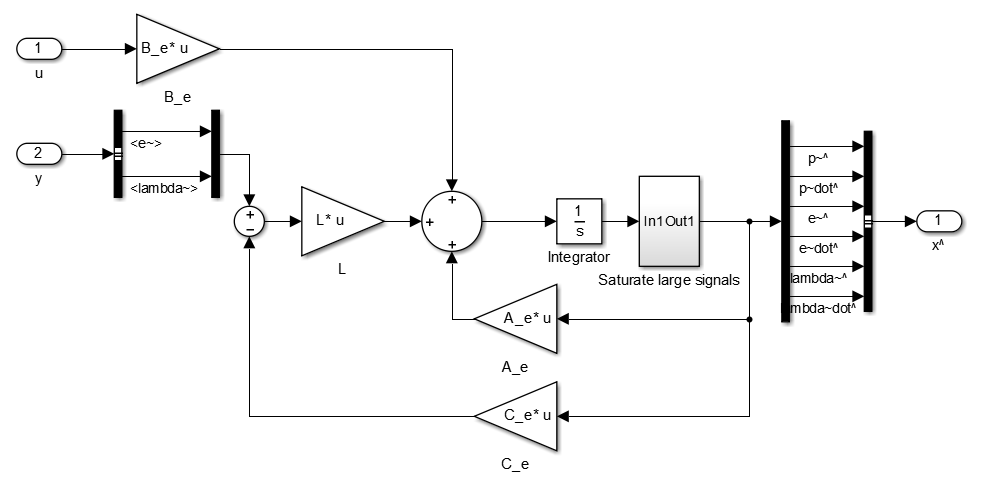
\includegraphics[scale=.6]{images/StateEstimator2States.png}
	\label{fig:Estimator 2 State}
\end{figure}

The observer gain matrix $\bm{L}$ is to be set in such a way that the
poles of the observer are faster than the system, in order to drive the
error to zero.
\begin{figure}[H]
  \caption{ illustrating how to place poles during state, or estimated
    state feedback, on a semi-circle with the same radius, within the
    region shown.}
  \label{fig:pole_placement}
  \begin{center}
    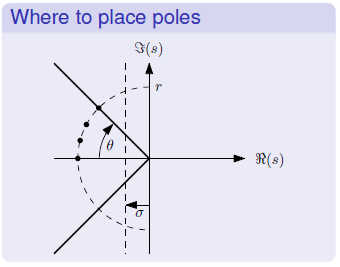
\includegraphics[width=0.5\textwidth]{images/pole_placement}
  \end{center}
\end{figure}
\todo[inline]{Finn navnene på theta og sigma i forhold til regtek} It is recommended that the
poles of the observer be placed as in
\cref{fig:pole_placement}. The real value of the observer poles must be larger
than $\sigma$, which for the observer is the value of the largest real
value of the controlled systems poles. This way, all of the linear
observers poles are such that the observer is faster than the controlled system. $\theta$ is the
largest angle of the observer poles. If this is too large, the system will be underdamped and cause
overshoots in the estimate. However, if the radius is too large, undesired high
frequency noise from the measurements becomes amplified to unwanted
levels. Furthermore, the observer will become increasingly unstable the closer the poles are.

$\theta = 15$, and $r$ as 50 times the maximum length of the
controlled systems poles worked well for this system.

The observer itself has the state space formulation:

\begin{equation*}
  \dot{\hat{\bm{x}}} = \bm{A}\hat{\bm{x}}+\bm{B}\bm{u} + \bm{L}(\bm{y}
  - \bm{C}\hat{\bm{x}})
\end{equation*}
\begin{align*}
  \dot{\bm{e}} &= \dot{\bm{\tilde{x}}} - \dot{\hat{\bm{x}}} \\
               &= \bm{Ax} + \bm{Bu} - \bm{A}\hat{\bm{x}} - \bm{Bu} - \bm{L}(\bm{y}- \bm{C}\hat{\bm{x}}) \\
               &= \bm{A}(\bm{x} - \hat{\bm{x}}) - \bm{L}(\bm{C}\bm{x}- \bm{C}\hat{\bm{x}}) \\
               &= \bm{Ae} - \bm{LCe} \\
\end{align*}
Meaning the error has the state space formulation:
\begin{equation}
  \dot{\bm{e}} = (\bm{A} - \bm{LC})\bm{e}
\end{equation}
As previously stated, for this error to converge to zero the poles of this state space formulation should be placed such that they are
faster than the poles of the system itself. The poles of this state
space system can be placed arbitrarily because $\{\bm{A},\bm{C}\}$ is
observable:
\begin{equation*}
  det(\lambda\bm{I} - \bm{A} +\bm{LC}) = 0
\end{equation*}
For this equation, $\lambda$ are the values that solves the equation,
and also the poles of the observer. By choosing values for $\lambda$,
an $\bm{L}$ emerges in order to make the determinant equal to
zero. The matlab function $place$ places the poles as desired for us:

$\bm{L} = place(\bm{A}^T,\bm{C}^T,\bm{\lambda})^T$, where
$\bm{\lambda}$ is the vector of the observer poles in this instance.

In \cref{fig:LQR_Estimator} the poles are palced on the real line at -20, -40, -60, -80, -100, and -120. This type of observer has minimal overshoot, as there are no complex parts, and the poles are spread far apart to avoid unstable behavior from the observer. Furthermore, the maximum radius is also rather large leading to a fast response. Placing the poles on the real line like this was slightly better than placing them evenly on a circle with radius $r = 60$, and an angle $\theta = 22.5$, because with this pole setup the observer was too oscillatory.
\todo[inline]{This r and theta are different than the one mentions previously (about 2 paragraphs back}

\newgeometry{left=0.5cm,right=0.5cm,top=1cm,bottom=2cm}
\begin{figure}
  \caption{LQR Controller Estimating $p, e$ and $\lambda$}
  \makebox[\textwidth][c]{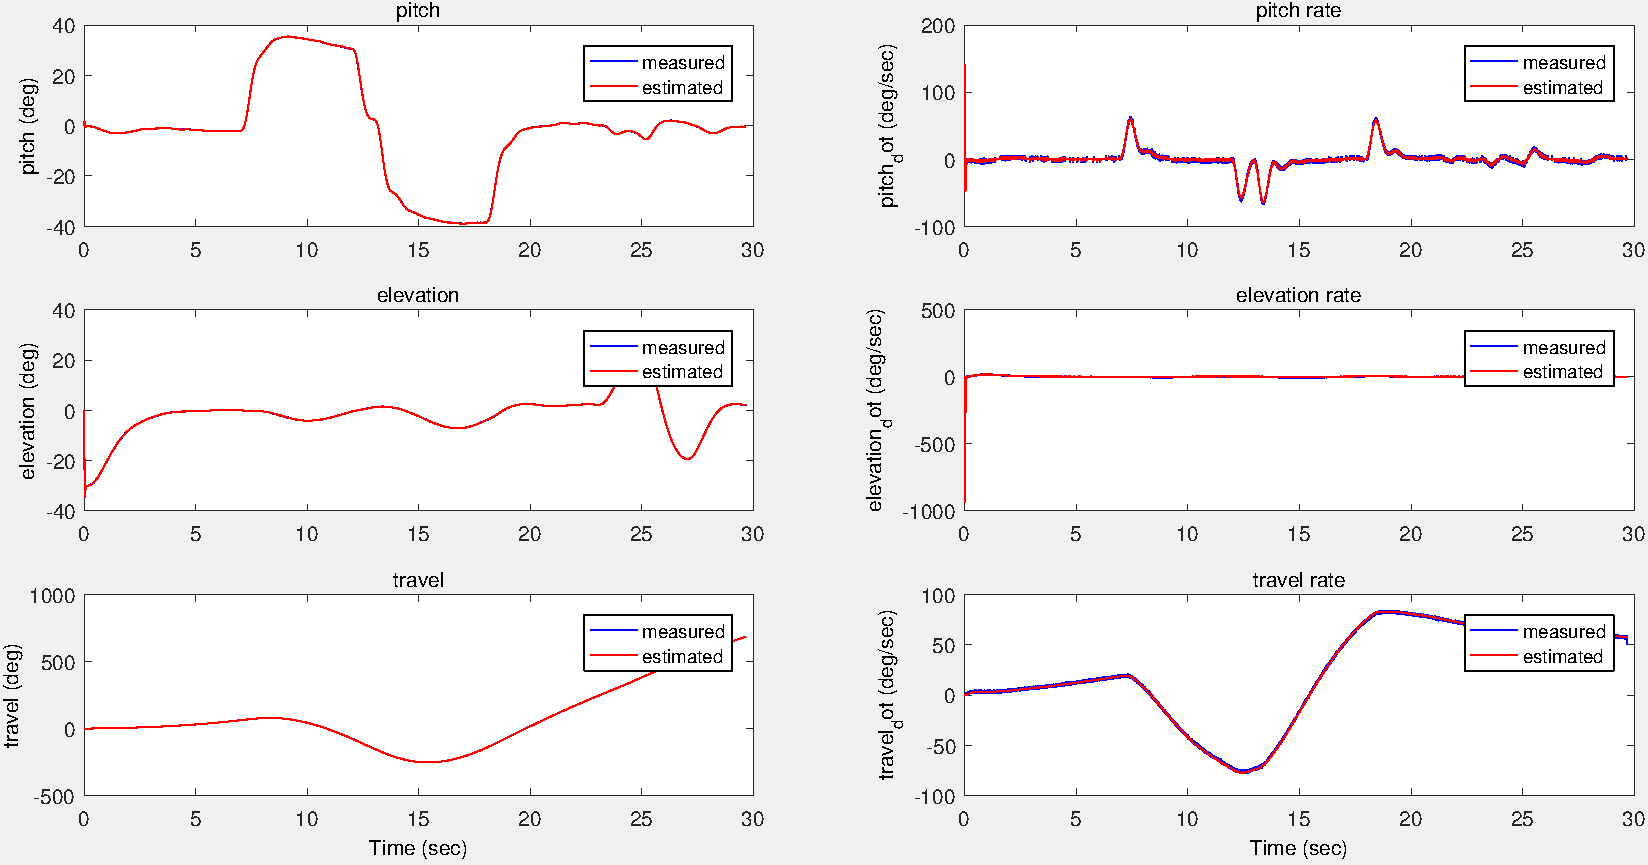
\includegraphics[width = \textwidth]{images/542_LQR_Estimator.pdf}}
  \label{fig:LQR_Estimator}
\end{figure}

\begin{figure}[p]
  \caption{LQR Controller with Integral Effect Estimating $p, e$ and $\lambda$}
  \makebox[\textwidth][c]{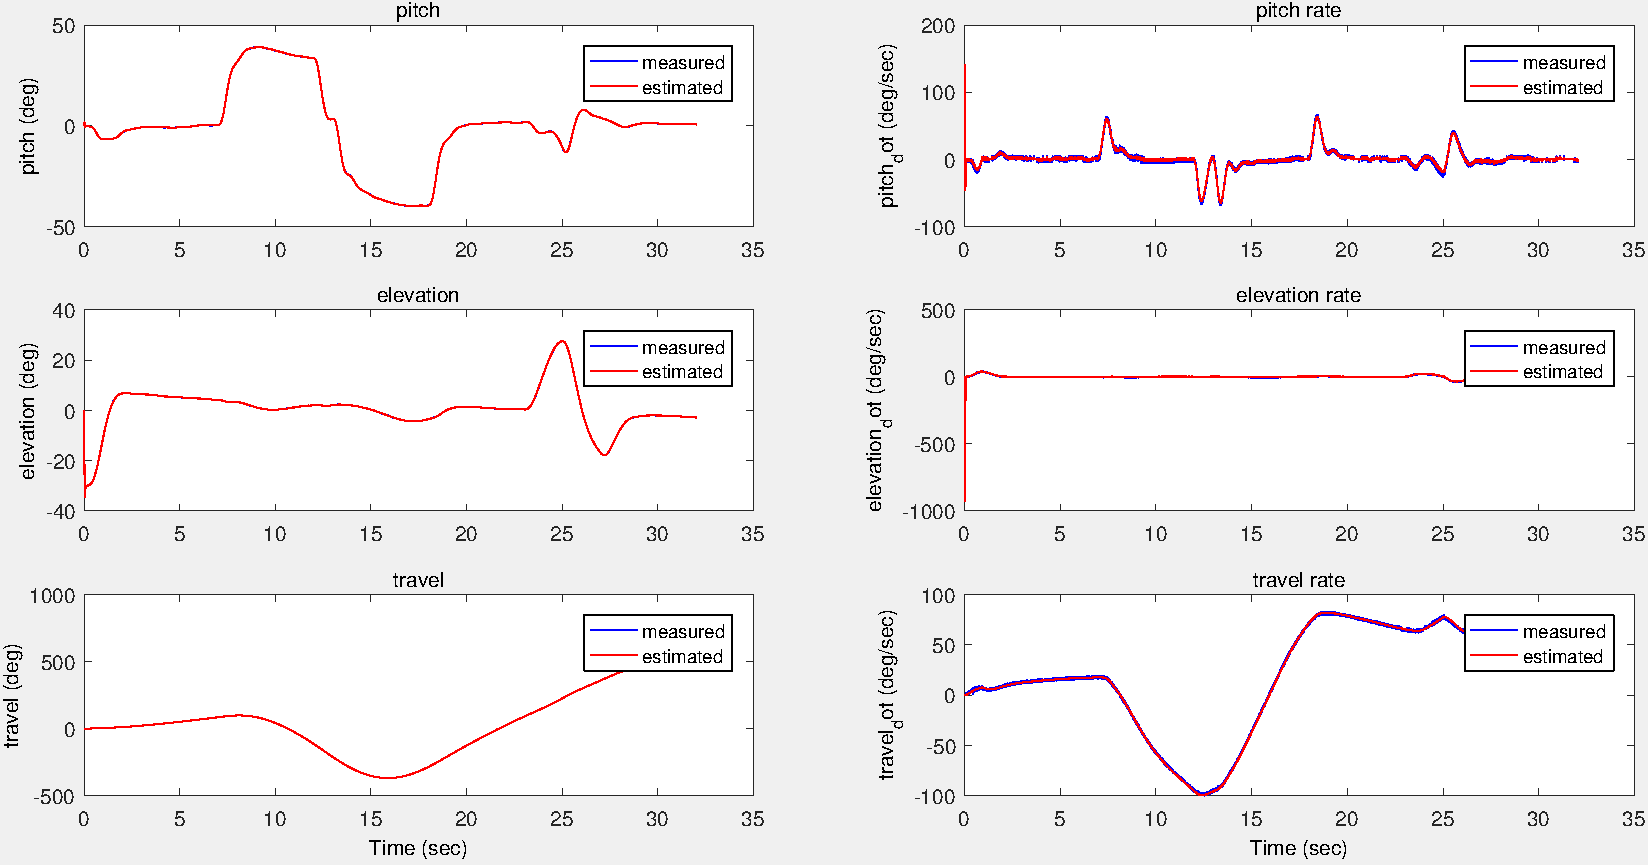
\includegraphics[width = \textwidth]{images/542_LQRIntegralEffect_Estimator.pdf}}
  \label{fig:LQRIntegralEffect_Estimator}
\end{figure}
\restoregeometry

\newgeometry{left=0.5cm,right=0.5cm,top=1cm,bottom=2cm}
\begin{figure}
  \caption{LQR Controller Estimating $p, e$ and $\lambda$}
  \makebox[\textwidth][c]{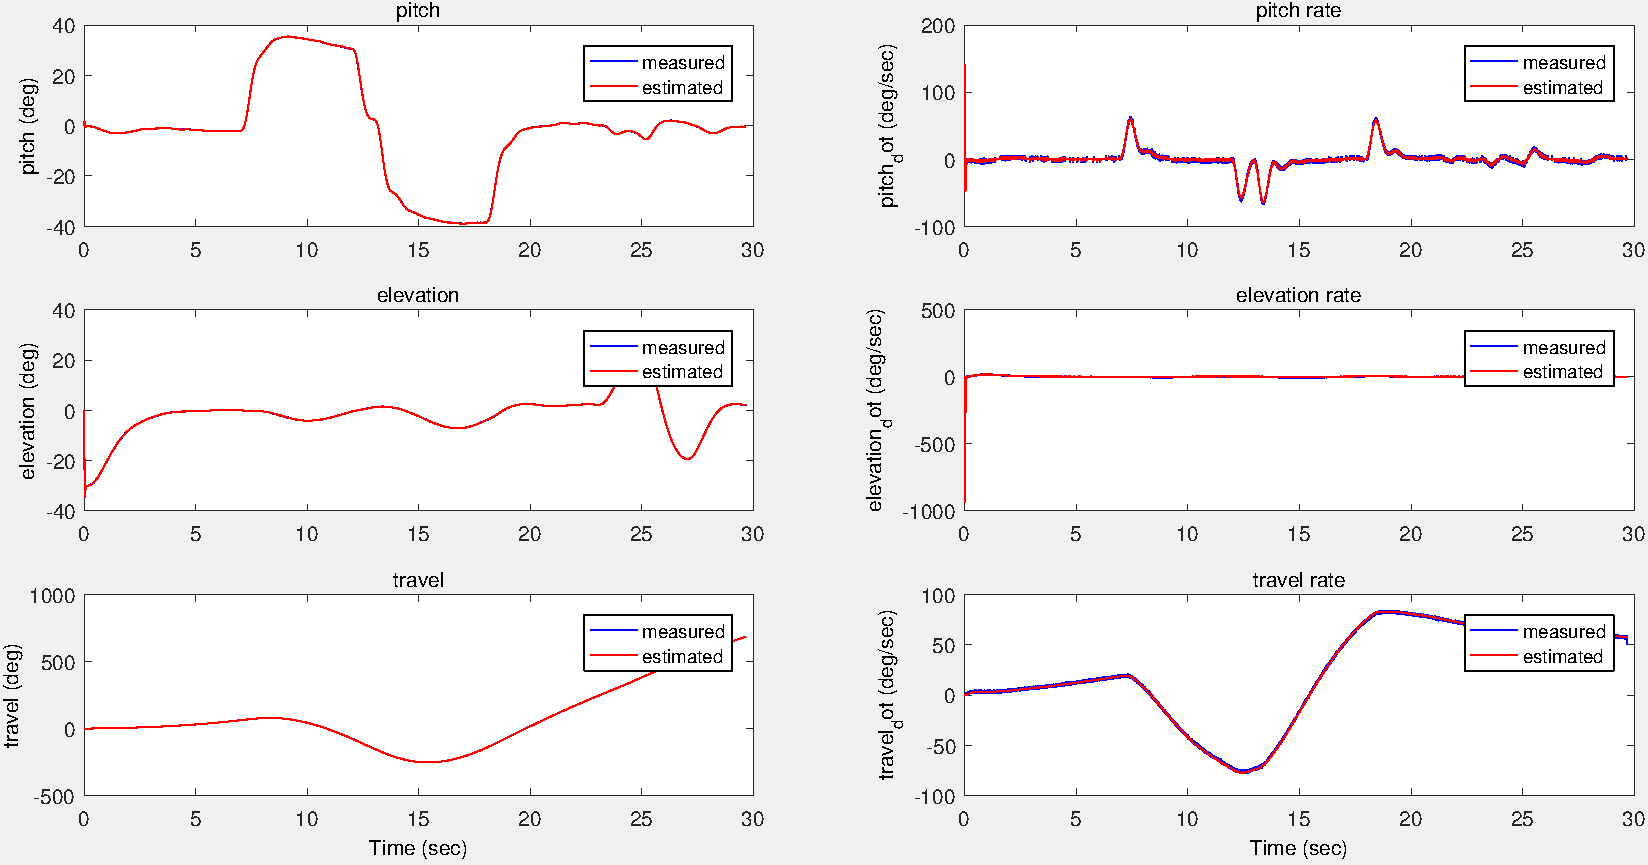
\includegraphics[angle=90, height = \textheight]{images/542_LQR_Estimator.pdf}}
  \label{fig:LQR_Estimator}
\end{figure}

\begin{figure}[p]
  \caption{LQR Controller with Integral Effect Estimating $p, e$ and $\lambda$}
  \makebox[\textwidth][c]{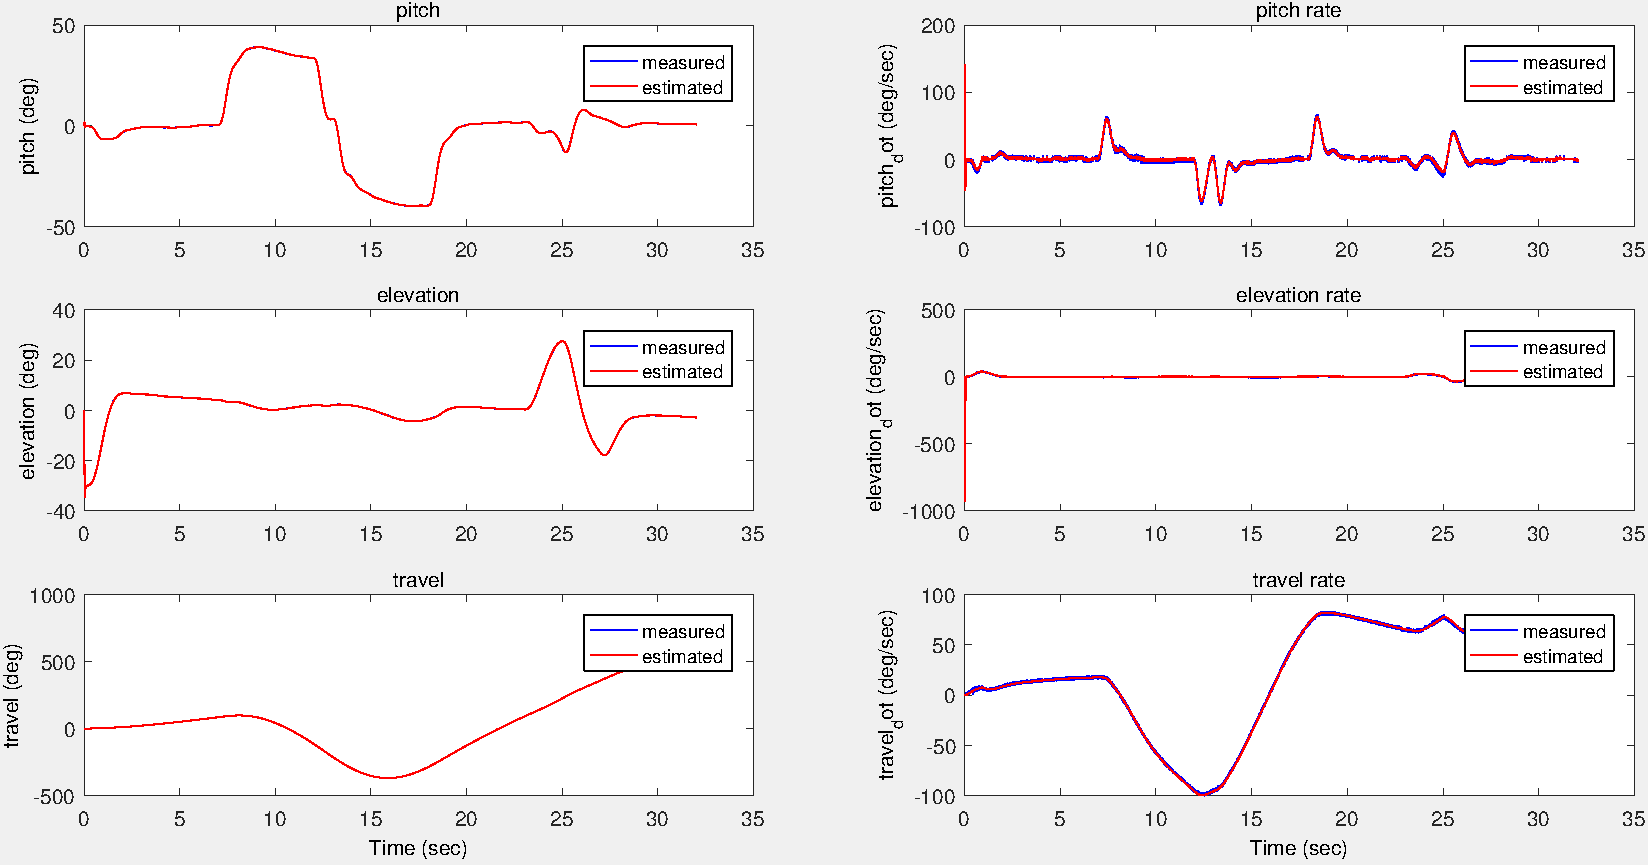
\includegraphics[angle = 90, height = \textheight]{images/542_LQRIntegralEffect_Estimator.pdf}}
  \label{fig:LQRIntegralEffect_Estimator}
\end{figure}
\restoregeometry

\subsection{Problem 3}

When only $\tilde{e}$ and $\tilde{\lambda}$ are measured, the output
matrix becomes:
%
\begin{equation*}
  \bm{C} =
  \begin{bmatrix}
    0 & 0 & 1 & 0 & 0 & 0 \\
    0 & 0 & 0 & 0 & 1 & 0
  \end{bmatrix}
\end{equation*}
%
The observer matrix, found through $obsv(\bm{A},\bm{C})$ is a 12x6
matrix with rank 6. Therefore, it is observable.

However, when only $\tilde{p}$ and $\tilde{e}$ are measured, the
output matrix becomes:
%
\begin{equation*}
  \bm{C} =
  \begin{bmatrix}
    1 & 0 & 0 & 0 & 0 & 0 \\
    0 & 0 & 1 & 0 & 0 & 0
  \end{bmatrix}
\end{equation*}
%
The observer matrix, found through $obsv(\bm{A},\bm{C})$ is a 12x6
matrix with rank 4. Therefore, it is not observable.

Quicknotes: tried one pole close to the system poles, and the rest out but close to the real line.
Noticed an underdamped behaviour of the elevation rate, estimate was slightly higher than the true state.
Tried complex conjugated poles slightly further out of the real line, got a much better response.

More notes: Larger observer poles also means larger $\bm{u}$ values

This observer is particularly challenging to implement due to the fact that pitch is measured based on the travel rate, which is based on travel. This means the estimator has to filter out two layers of measurement noise. This means that choosing the observer poles becomes difficult because as the radius of the poles increases it begins to amplify this noise.

\newgeometry{left=0.5cm, right=0.5cm, top=1cm, bottom=2cm}
\begin{figure}[h]
\caption{Output using Estimator that measures elevation and travel}
\makebox[\textwidth][c]{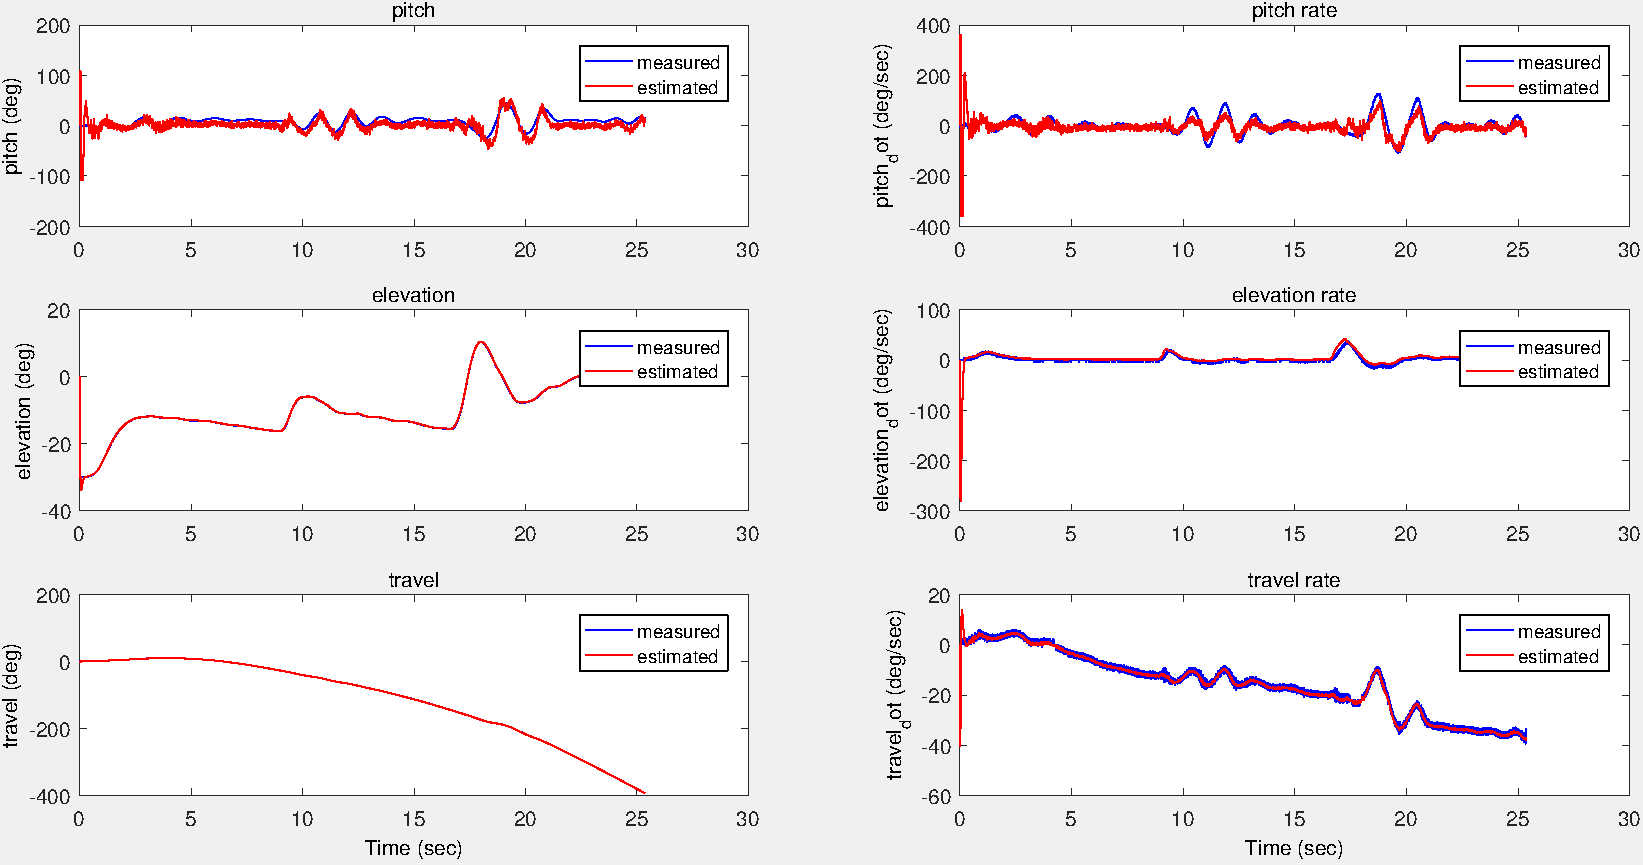
\includegraphics[angle=90, height=\textheight]{images/543_Estimator}}
\label{fig:Estimator4_3}
\end{figure}


%%% Local Variables:
%%% mode: latex
%%% TeX-master: "report_main"
%%% End:

\newpage
%%% Local Variables:
%%% mode: latex
%%% TeX-master: "report_main"
%%% End:

\begin{thebibliography}{9}
\bibitem{chen14}
  Chi-Tsong Chen,
  \emph{Linear System Theory and Design},
  Oxford University Press,
  4th edition,
  2014

\bibitem{assignment}
  Kristoffer Gryte et al.,
  \emph{Helicopter lab assignment},
  Department of Engineering Cybernetics,
  NTNU,
  Version 4.5,
  2015

\bibitem{lecture5}
  Morten D. Pedersen,
  \emph{TTK4115 Lecture 5 State Feedback},
  Department of Engineering Cybernetics,
  NTNU,
  19.09.2016
	
\end{thebibliography}

\end{document}
